%----------------------------------------------------------------
%---------------------- Anexos ----------------------------------
%----------------------------------------------------------------

\begin{anexosenv}
%\partanexos   % indica o início dos anexos
\chapter{Mapa de unidades do IFMG.}
\label{anexoA}

Note que os  Anexos são  \textbf{documentos  que não foram  elaborados  pelo  autor},  que  servem  também  de  fundamentação, comprovação ou ilustração do trabalho, como leis, mapas, ilustrações etc .

\begin{figure}[H] % h! para here, b para bottom e t para top
   \begin{center}
    \caption{Mapa de unidades do IFMG.} %//não esqueça o ponto final
    \label{fig:mapas}
    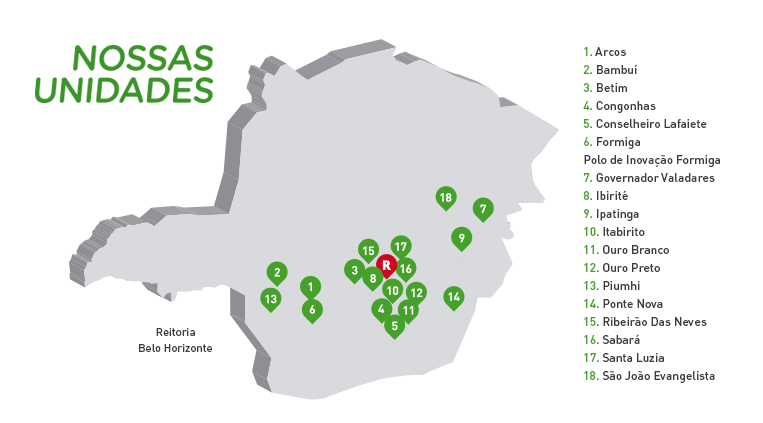
\includegraphics[width=1\linewidth]{Figuras/mapasitenovonov2018b.png} \\
    \end{center}
    \fontsize{10}{12}\selectfont{Fonte: \href{https://www.ifmg.edu.br/portal/sobre-o-ifmg/mapasitenovonov2018b.png}{https://www.ifmg.edu.br/portal/sobre-o-ifmg}. }
\end{figure}



\end{anexosenv}
